\documentclass{article}

\usepackage[accepted]{icml2023}

% Packages
\usepackage{hyperref}
\usepackage{graphicx}
\usepackage{booktabs}
\usepackage{multirow}
\usepackage{amsmath}
\usepackage{xcolor}
\usepackage{subcaption}
\usepackage{listings}
\usepackage{float}
\usepackage{tcolorbox}
\usepackage{algorithm, algpseudocodex}
\usepackage{epstopdf}

% Graphics
\DeclareGraphicsExtensions{.png,.pdf}

% Aliases
\newcommand{\github}{\href{https://github.com/mikasenghaas/diloco-swarm}{GitHub}}
\newcommand{\wandb}{\href{https://wandb.ai/mikasenghaas/diloco-swarm}{Weights \& Biases}}
\newcommand{\gist}{\href{https://gist.github.com/mikasenghaas/5fa1aa77ea69f187f531a5889983c249}{GitHub Gist}}

% Colors
\definecolor{bblue}{HTML}{5884E2}
\definecolor{oorange}{HTML}{F19E38}
\definecolor{ppurple}{HTML}{9900FF}

% Colored boxes
\newcommand{\orangebox}{\colorbox{oorange!50}{\hspace{0.3em}}}
\newcommand{\bluecircle}{\textcolor{bblue}{\LARGE$\bullet$}}
\newcommand{\purplecircle}{\textcolor{ppurple}{\LARGE$\bullet$}}

% Code
\definecolor{codegreen}{rgb}{0,0.6,0}
\definecolor{codegray}{rgb}{0.5,0.5,0.5}
\definecolor{codepurple}{rgb}{0.58,0,0.82}
\definecolor{backcolour}{rgb}{0.95,0.95,0.95}
\lstdefinestyle{mystyle}{
    backgroundcolor=\color{backcolour},   
    commentstyle=\color{codegreen},
    keywordstyle=\color{magenta},
    numberstyle=\tiny\color{codegray},
    stringstyle=\color{codepurple},
    basicstyle=\ttfamily\footnotesize,
    showspaces=false,                
    showstringspaces=false,
    showtabs=false,                  
    tabsize=2
}
\lstset{style=mystyle}

% Running Title
\icmltitlerunning{DiLoCo-SWARM}


\begin{document}

\begin{titlepage}
\begin{center}
    \Large{\textsc{École Polytechnique Fédérale de Lausanne}}\\
    \vspace{1cm}
    
\includegraphics[width=5cm]{figures/epfl.png}
    \vspace{1cm}
    
    \large{Optional Master Research Project, \textit{January 2025}}\\
    
    \vspace{1cm}
    \rule{\textwidth}{1pt}\vspace{15pt}
    \Huge{DiLoCo-SWARM}
    \rule{\textwidth}{1pt}
    
    \vspace{1cm}
    
    \large{\textsc{Mika SENGHAAS}\\\texttt{mika.senghaas@epfl.ch}}
    \vspace{\stretch{1}}
    
    \large{
      \textit{Supervisors}\\
      \textsc{Martijn DE VOS}, \textsc{Akash DHASADE}, \textsc{Rishi SHARMA}}\\
      \vspace{0.5cm}
      \textit{Professor}\\
      \textsc{Anne-Marie KERMARREC}\\
      \vspace{0.5cm}
      \large{\textit{Laboratory}\\
      Scalable Computing Systems (SaCS)\\
    }
\end{center}
\end{titlepage}

% Title
% \twocolumn[
%   \icmltitle{DiLoCo-SWARM}
%   \begin{icmlauthorlist}
%     \icmlauthor{Mika Senghaas}{author}
%     \icmlauthor{Martijn De Vos}{supervisor}
%     \icmlauthor{Akash Dhasad}{supervisor}
%     \icmlauthor{Rishi Sharma}{supervisor}
%   \end{icmlauthorlist}
%   \icmlaffiliation{author}{Author}
%   \icmlaffiliation{supervisor}{Supervisor}
%   \icmlcorrespondingauthor{Mika Senghaas}{mika.senghaas@epfl.ch}
%   \icmlkeywords{Distributed Training, Decentralized AI, SWARM, DiLoCo}
%   \vskip 0.3in
% ]
% \printAffiliationsAndNotice{}

% Abstract
\begin{abstract}
  We investigate DiLoCo-SWARM, a decentralized training approach that combines
  the pipeline and data parallelism of SWARM with DiLoCo's reduced-frequency
  gradient synchronization. Our experiments on language modeling tasks show that
  DiLoCo-SWARM matches or surpasses fully synchronized SWARM baselines despite
  synchronizing gradients up to 50 times less frequently.
\end{abstract}

\section{Introduction}

% Centralized training
Modern foundation models have billions of parameters and are trained on
trillions of
tokens~\cite{chowdhery2022palm,brown2023gpt3,dubey2024llama3,google2024gemini}.
Operating at such scale requires orchestrating thousands of GPUs to distribute
computation~\cite{dubey2024llama3,deepseekai2024}. However, traditional
parallelization techniques rely on fast interconnect to not bottleneck the
training. Hence, frontier-scale models are currently trained in high performance
clusters (HPC). Operating HPCs is costly, leaving research capabilities to a
small number of corporate and state entities~\cite{jaghouar2024intellect1}. 

% This creates significant points of control, and in turn increases the risk of
% capability capture or misue.

% Decentralized training
Recently, decentralization has emerged as a promising counter-weight to this
trajectory. Decentralized training aims to pool the vast, cheap compute
resources across the globe for collaborative model training efforts. However,
this new paradigm brings significant technical and algorithmic challenges. Most
prominently, training algorithms have to accomodate orders-of-magnitude slower
interconnect, hetereogeneous compute pools, and nodes dynamically joining or
leaving the training. 
% TODO: Potentially remove dynamic world size to focus on fitting larger models

% Intellect-1 and DiLoCo
For this reason, current decentral training efforts can not yet match the scale
and efficiency of the centralized setting. Yet, the field is progressing rapidly
and gaining interest in the research community.
INTELLECT-1~\cite{jaghouar2024intellect1} is the most recent demonstration that
large-scale decentral model training is possible. It is a 10B parameter model
trained across three continents. The model is a scale-up of
DiLoCo~\cite{douillard2023diloco}, a low-cost communication distributed data
parallel (DDP) training method. Compared to traditional DDP, DiLoCo's key
insight is to replace regular gradient synchronization at every step with less
frequent synchronization using a dual optimization scheme. Their empirical
results show that the method preserves performance while requiring a fraction of
the communication cost, i.e. only every 500 steps. The experiments have since
been replicated~\cite{jaghouar2024opendiloco}, and
scaled~\cite{jaghouar2024intellect1}, underlining the robustness of the
approach. However, like traditional data parallel training, a key limitation is
that each node has to store a full copy of the model to participate during
training. Further, in heterogeneous compute setups,  faster hardware is becomes
underutilized. Hence, only powerful 8xH100 GPU racks were allowed for training
INTELLECT-1.

% SWARM
SWARM~\cite{ryabinin2023swarm} parallelism is a promising, but less explored,
alternative for decentralized training that is designed for larger scale. Unlike
DiLoCo, which relies solely on data parallelism, SWARM combines two types of 
parallelism - data and pipeline parallel. By also sharding the model, SWARM can
scale to larger models, or vice versa, allow lower-end devices to participate in
training. This makes it an attractive candidate for further scaling
decentralized training efforts. In its original formulation, SWARM requires
gradient synchronization between all nodes serving the same pipeline stage of a
model. 

% DiLoCo-SWARM
The above two approaches motivate this research, which investigates whether
step-wise gradient synchronization in SWARM pipeline stages can be replaced by
DiLoCo-style synchronization. We term this method DiLoCo-SWARM. Our key findings
and contributions can be summarized as follows:

% TODO: Maybe mention results from ablations
\begin{enumerate}
  \item \textbf{DiLoCo-SWARM.} We show that SWARM parallelism is compatible with
  DiLoCo-style gradient synchronization. While requiring \textit{50x fewer
  gradient updates}, we obtain a validation perplexity of \textit{30.15},
  exceeding the synchronous baseline of \textit{30.22}.
  \item \textbf{Implementation.} We release a minimal training script
  implementing a feature subset of SWARM parallelism, as well the DiLoCo
  optimizer. Instead of multiple thousands, the implementation uses a few
  hundred lines of pure PyTorch code.
\end{enumerate}

Besides open-sourcing the full experiment code and results on \github{} and
\wandb{}, we release a distilled version of the training logic as a \gist{}. We
hope that these resources will serve as a starting point for further open-source
research efforts with SWARM, and spark interest in scaling SWARM from research
to production-grade systems, similarly to the development of DiLoCo.

\section{Background}

\subsection{Distributed Training}

In distributed training, $n$ nodes collaboratively train a \textit{model}
$f_{\theta}$ parameterized by weights $\theta$, on a \textit{dataset} of samples
$D = \{(\mathbf{x}_1, \mathbf{y}_1),\dots\}$. Collaboration requires nodes to
periodically communicate intermediate results. We will describe two popular
parallelization techniques relevant in the context of DiLoCo-SWARM.

\begin{figure}[ht]
    \centering
    \begin{subfigure}[b]{0.48\textwidth}
        \centering
        \vspace{0.5cm}
        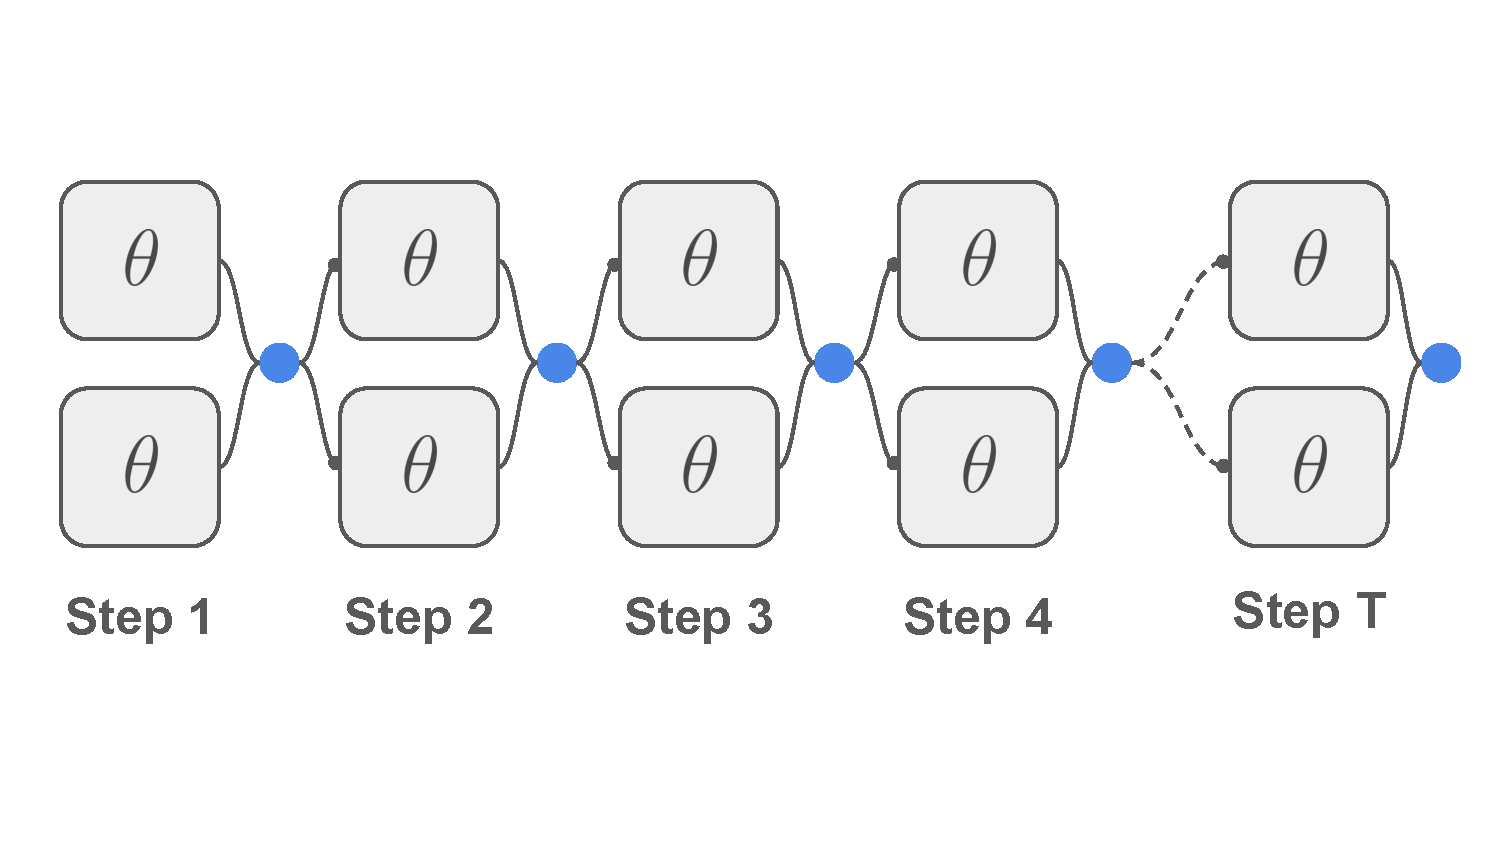
\includegraphics[width=\textwidth]{figures/dp.pdf}
        \caption{\textbf{Data Parallelism.} In DP, nodes synchronize (\bluecircle) local gradients at every step using an \texttt{AllReduce}
        operation.}
        \label{fig:dp}
    \end{subfigure}
    \hfill
    \begin{subfigure}[b]{0.45\textwidth}
        \centering
        \vspace{0.5cm}
        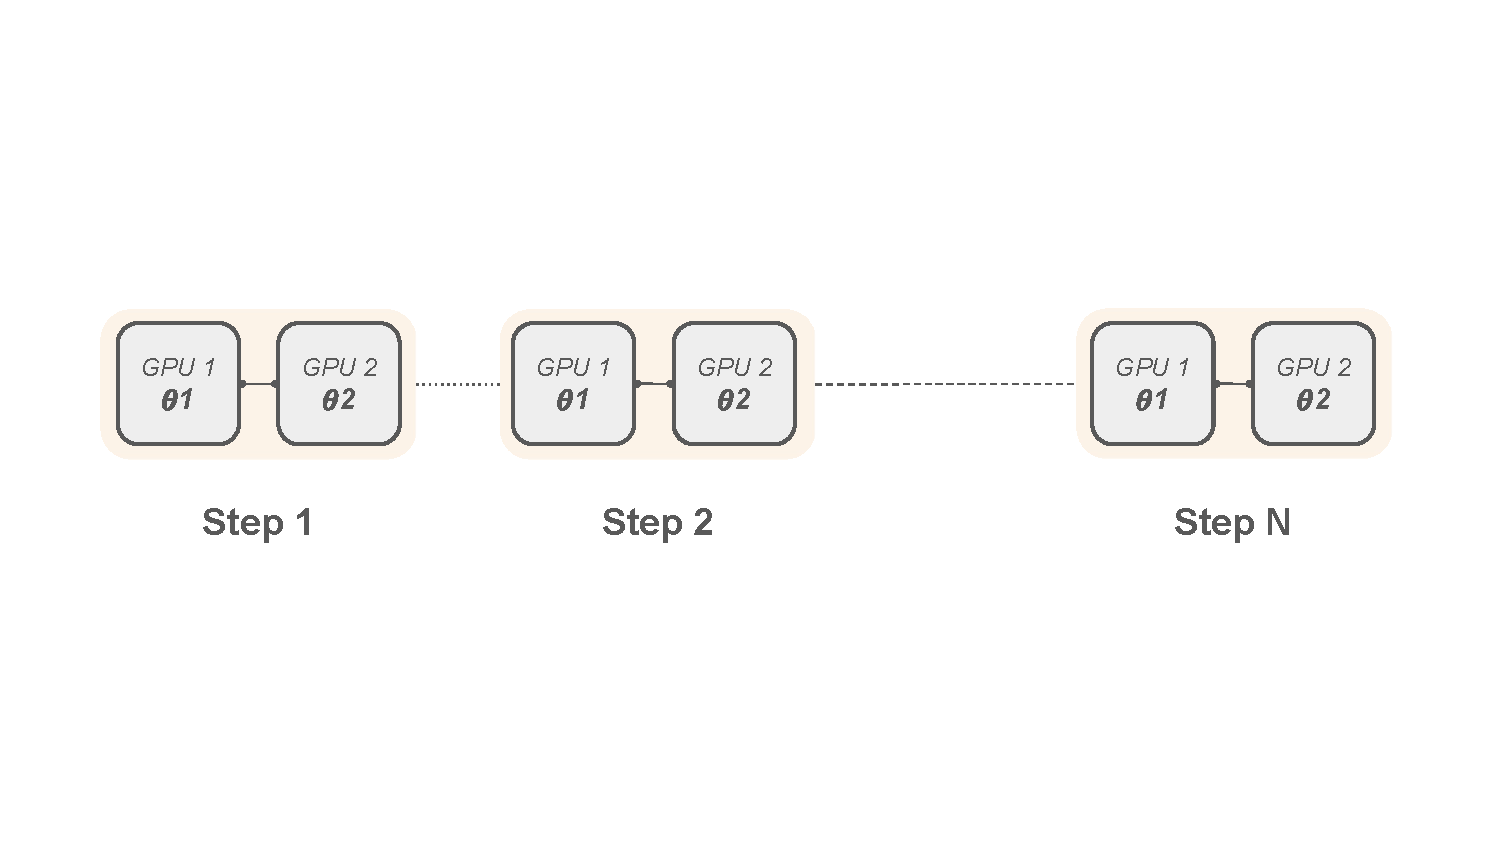
\includegraphics[width=\textwidth]{figures/pp.pdf}
        \caption{\textbf{Pipeline Parallelism.} In PP, nodes communicate
        activations and gradients (\orangebox) between adjacent stages.}
        \label{fig:pp}
    \end{subfigure}
    \caption{\textbf{DP and PP.} We show communication patterns for $n=2$ DP and
    PP groups over $T$ training steps. Nodes are represented as boxes,
    communication as solid lines. Dotted lines indicate no communication.}
\end{figure}

\textit{Data parallelism} (DP)~\cite{dean2012dp} partitions the dataset,
creating $n$ data shards $D_1,\dots,D_n$. The $i$-th node holds a local data
shard $D_i$ and a copy of the full model parameters $\theta$. Training proceeds
as shown in Algorithm~\ref{alg:dp}: First, each node samples a batch from its
data shard and computes local gradients via a full forward and backward pass.
Next, all nodes average their local gradients into an identical global gradient
and perform the same model update. The all-to-all communication, as visualized
in Figure~\ref{fig:dp}, is typically enabled by an
\texttt{AllReduce}~\cite{walker1995mpi} operation.

% DP communication becomes costlier as the number of model parameters and nodes increases.

\begin{algorithm}
\caption{Data Parallel Gradient Synchronization}
\label{alg:dp}
\begin{algorithmic}[1]
\State {\bfseries Input:} Local Dataset $D_i$, Model $\theta^{(t-1)}$, Optimizer $\mathtt{OPT}$, Loss $\mathcal{L}$
\State Sample batch: $x_i\sim D_i$
\State Compute gradient: $g_i \gets \nabla_{\theta^{(t-1)}} \mathcal{L}(x_i; \theta^{(t-1)})$
\State Sync gradients: $g \gets \frac{1}{n}\sum_{i}^n g_i$ \Comment{$\mathtt{AllReduce}$}
\State Update model: $\theta_i^{(t)} \gets \mathtt{OPT}(\theta^{(t-1)}, g)$
\end{algorithmic}
\end{algorithm}

\textit{Pipeline parallelism} (PP)~\cite{huang2019gpipe} partitions the model,
creating $n$ model shards $f^{(1)},\dots,f^{(n)}$ parameterized by
$\theta_1,\dots,\theta_n$, such that the full model is represented as a pipeline
of form $f_{\theta}=f^{(1)}_{\theta_1}\circ\dots\circ f^{(1)}_{\theta_n}$. Model
shards are often referred to as "stages" in the pipeline, where the $i$-th stage
serves the model shard $f^{(i)}_{\theta_i}$.  For deep learning architectures
such a layer-wise partition is natural, as they are typically architected as
repeated computational blocks, e.g. convolutional blocks in
CNNs~\cite{krizhevsky2012alexnet} and Transformer blocks in
Transformer~\cite{vaswani2017transformer} The partitioning creates a
bi-directional communication pattern between stages during training, as shown in
Figure~\ref{fig:pp}: During a forward pass activations are communicated from
stage $i$ to $i+1$, and during the backward pass gradients are sent from stage
$i$ to $i-1$. Despite its simplicity, PP is notoriously hard to optimize. Naive
implementations suffer from significant GPU idle time, e.g. when the first node
has to wait for the full pipeline forward and backward pass before being able to
compute its local gradient. Efficient PP implementations therefore rely on
micro-batching and advanced scheduling techniques to be practically
viable~\cite{harlap2018pipedream, huang2019gpipe}. 

% PP communication cost scales with the number of stages $n$, the micro batch size and the model's hidden dimension, but 

It is possible to design \textit{hybrid parallelism} (DPP) which combines DP and
PP. It is natural to partition both the dataset and model into $\{D_i\}_{i\in
[m]}$ and $\{\theta_j\}_{j\in [n]}$. This creates a $m\times n$ grid, where the
$(i,j)$-th node handles data shard $D_i$ and model shard $\theta_j$. The
emerging $m\times n$ grid structure is visualized for $9$ nodes distributed
evenly into three stages in Figure~\ref{fig:dpp}. The partition of model and
data results in independent PP ({\color{oorange} PP1, PP2, PP3}) and DP
({\color{bblue} DP1, DP2, DP3}) groups, shown as shaded areas. During training,
the communication patterns are interleaved: First, nodes send activations and
gradients (PP communication) within each PP group $i=1\dots,m$ to accumulate
local gradients. Then, within each DP group $j=1,\dots,n$, nodes run an
\texttt{AllReduce} to average local gradients for their model shard (DP
communication). 

\begin{figure}[ht]
    \centering
    \vspace{0.5cm}
    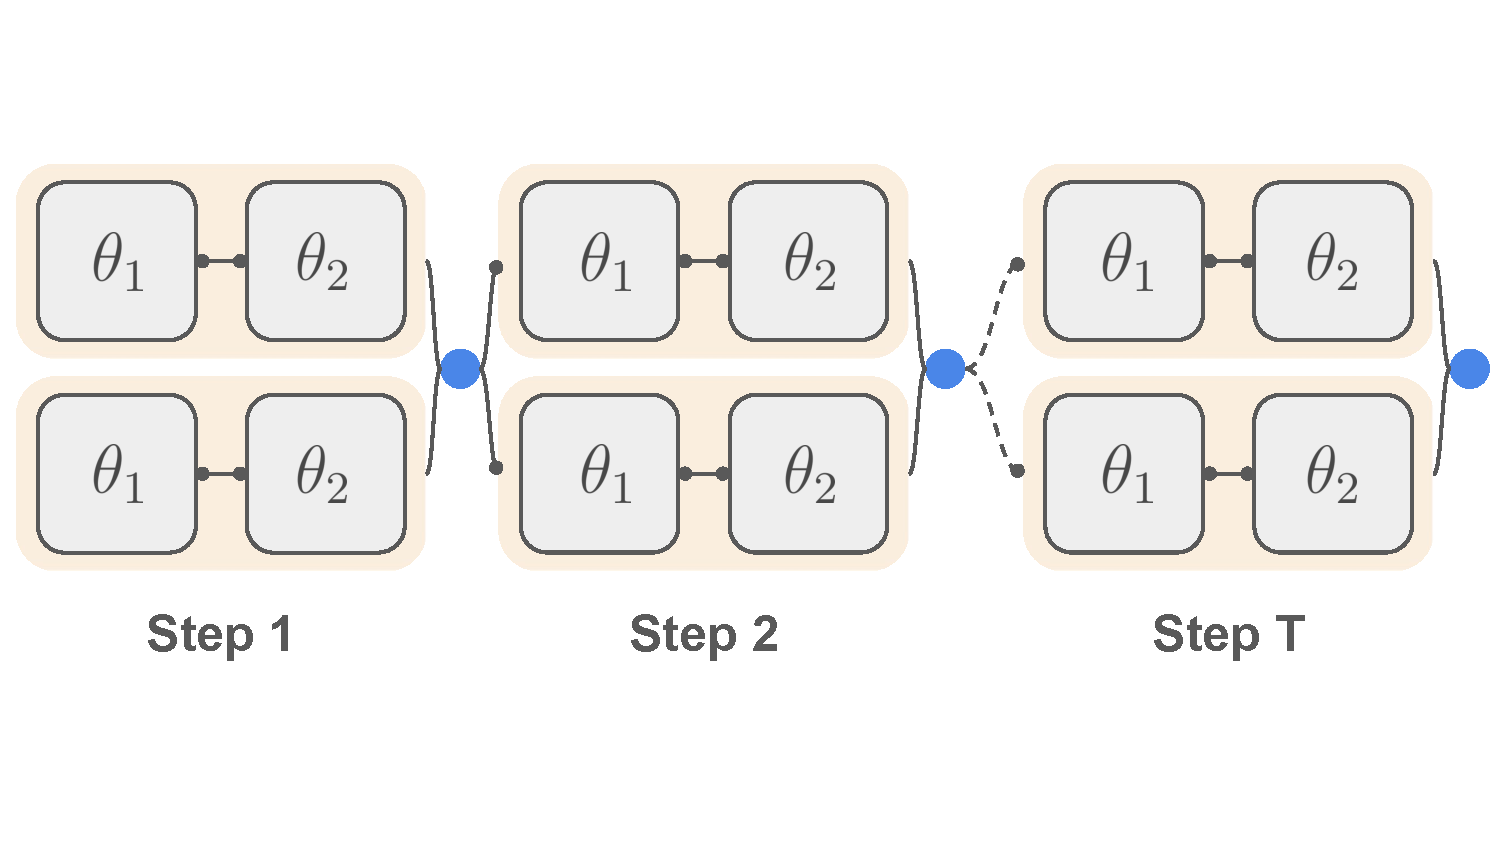
\includegraphics[width=0.48\textwidth]{figures/dpp.pdf}
    \caption{\textbf{DPP.} We show communication patterns in a 2D grid of
    $2\times2$ nodes over $T$ training steps. PP and DP communication is
    interleaved.  First, nodes accumulate gradients by forward and backward
    passes through pipelines in independent PP groups (\mbox{\orangebox}). Then,
    they average gradients in DP groups (\mbox{\bluecircle}) before performing a
    model update.}
    \label{fig:dpp}
\end{figure}

All described parallelization techniques produce equivalent gradient updates,
leading to identical models $\theta^{(t)}$ at any $t$. However, they
fundamentally differ in how they distribute computation across nodes and create
distinct communication patterns, as described. Even in centralized settings,
identifying the optimal parallelization technique is complex as it is highly
sensitive to the model size, as well as training, hardware and network
setup~\cite{hagemann2024parallelization, fernandez2024scalingtrends}.

% \subsection{Decentralized Training}
% 
% Decentralized training may be viewed a special form of distributed training
% subject to additional constraints imposed by typical hardware and network
% conditions in globally distributed node pools.
% 
% \begin{enumerate}
%   \item \textit{Slow Interconnect:} The average bandwidth is typically
%   orders-of-magnitude lower than in typical HPC settings.
%   \item \textit{Network Heterogenity:} Interconnect may vary greatly between
%   different pair of nodes, resulting in asymmetric communication.
%   \item \textit{Device Heterogenity:} Devices may range from low-end to high-end
%   \item \textit{Dynamic World Size:} Devices may leave or enter the training at any time
% \end{enumerate}
% 
% In this setting, traditional parallelization methods become
% \textit{communication-bound}. This means that the majority of the training time
% is spent waiting for networking operations to follow, leading to low device
% utilization.  It follows that such systems are not scalable, as adding more or
% better compute simply results in more idle time. Decentralized settings
% therefore require algorithmic innovations that make traditional methods more
% scalable.

\subsection{DiLoCo}

In the decentralized setting synchronizing gradients every step
(Algorithm~\ref{alg:dp}) may be prohibitive due to slow interconnect.
DiLoCo~\cite{douillard2023diloco} adapts traditional DP to the decentral
setting by significantly reducing the required synchronization frequency. It is
based on a local-global optimization scheme, described in
Algorithm~\ref{alg:diloco}. Each worker $i=1,\dots,n$ in a world of
$n$ nodes has access to a local data shard $D_i$ and stores a full model replica
$\theta$. Training proceeds by each node training locally for a fixed number of
$H$ steps using a local optimizer. To synchronize, each node computes and
averages its pseudo-gradient (the difference between the parameters before and
after the inner optimization) to update a global model using an global
optimizer. Training proceeds iteratively, starting from the shared global model.

\begin{algorithm}
\caption{DiLoCo Gradient Synchronization}
\label{alg:diloco}
\begin{algorithmic}[1]
\State \textbf{Input:} Local dataset $D_i$, Model $\theta^{(t-1)}$, Optimizers $\mathtt{OPT}_{\text{local}}$ and $\mathtt{OPT}_{\text{global}}$, Loss $\mathcal{L}$, Num. Local Steps $H$ 
\State Copy global model: $\theta_i^{(t-1)} \gets \theta^{(t-1)}$
\For{$H$ steps}
  \State Sample batch: $x \sim D_i$
  \State Compute gradient: $g_i \gets \nabla_{\theta_i} \mathcal{L}(x_i; \theta_i^{(t-1)})$
  \State Update local model: $\theta_i^{(t-1)} \gets \mathtt{OPT}_{\text{local}}(\theta_i^{(t-1)}, g_i)$
\EndFor
\State Compute pseudo-gradient: $\Delta_i \gets \theta_i^{(t-1)} - \theta^{(t-1)}$
\State Sync pseudo-gradients: $\Delta \gets \frac{1}{n}\sum_i^n \Delta_i$ \Comment{$\mathtt{AllReduce}$}
\State Update global model: $\theta^{(t)} \gets \mathtt{OPT}_{\text{global}}(\theta^{(t-1)}, \Delta)$
\end{algorithmic}
\end{algorithm}

Figure~\ref{fig:diloco} compares DP and DiLoCo, visualizing the points of
synchrony throughout training. Clearly, DiLoCo reduces the communication cost by
a factor of $1/H$, allowing each node to independently perform its inner
optimization loop for $H$ steps. The key insight is that $H>>1$ without
negatively effecting generalization performance. Empirical
evidence~\cite{douillard2023diloco,jaghouar2024opendiloco} shows that DiLoCo
with $H=500$ local steps matches the generalization performance of a DP
baseline, i.e. we can obtain the same performance but with 500x less
communication. However, DiLoCo shares many challenges with traditional data
parallel training. Most notably, DiLoCo does not scale to models that do not fit
into the local workers' memory - relying on slow parameter offloading
methods~\cite{cui2016}, gradient quantization~\cite{jaghouar2024intellect1} and
other tricks for scaling.

\begin{figure}[ht]
    \centering
    \vspace{0.5cm}
    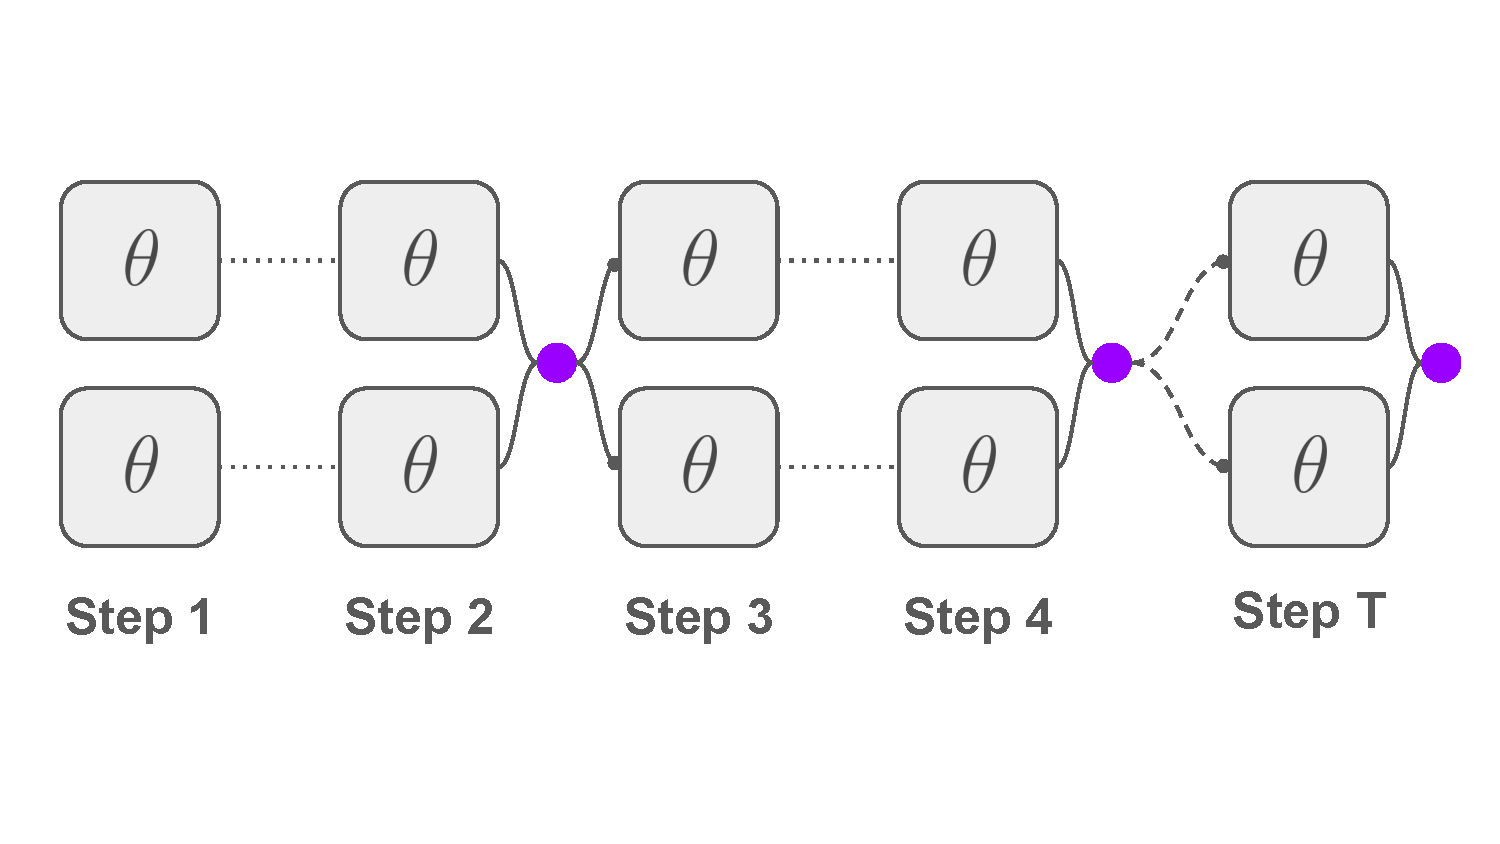
\includegraphics[width=0.45\textwidth]{figures/diloco.pdf}
    \caption{\textbf{DiLoCo.} We visualize communication patterns for a $n=2$
    DiLoCo group over $T$ training steps. Unlike DP, pseudo-gradients are
    synchronized (\purplecircle) every $H=2$ local steps, reducing the total
    communication cost by a factor of $1/2$.}
    \label{fig:diloco}
\end{figure}


\subsection{SWARM}

% TODO: Add square-cube law -> DP scales cubic, PP quadratic

Sharding the model is a natural solution to circumvent the memory limitations of
DP methods. However, traditional PP is not well suited for decentral settings.
Due to its inherently sequential nature, the pipeline is bottlenecked by its
weakest link (either device or network), leading to signifcant idle time for
faster nodes. Furthermore, a single node failure will stall the entire training
procedure.

SWARM parallelism~\cite{ryabinin2023swarm} proposes a fault-tolerant DPP
realization. Instead of organizing nodes in a rigid grid, SWARM constructs
stochastic pipelines on-the-fly, as illustrated in Figure~\ref{fig:swarm}.
During the forward pass, activations are forwarded to any peer in the subsequent
stage with probability proportional to each peer's throughput. During the
backward pass, gradients follow reversed paths, such that each node can
accumulate local gradients. Once all micro batches are processed, nodes within a
SWARM stage form DP groups, and synchronize their local gradients before
performing the model update. \textit{Stochastic wiring} has two benefits. On the
one hand, it naturally distributes workload even in heterogeneous compute and
network settings. On the other hand, it enables the SWARM pipeline to recover
from node failures by "re-wiring" lost activations or gradients. In this way,
SWARM remains functional as long as each stage is served by at least one node.
\begin{figure}[ht]
    \centering
    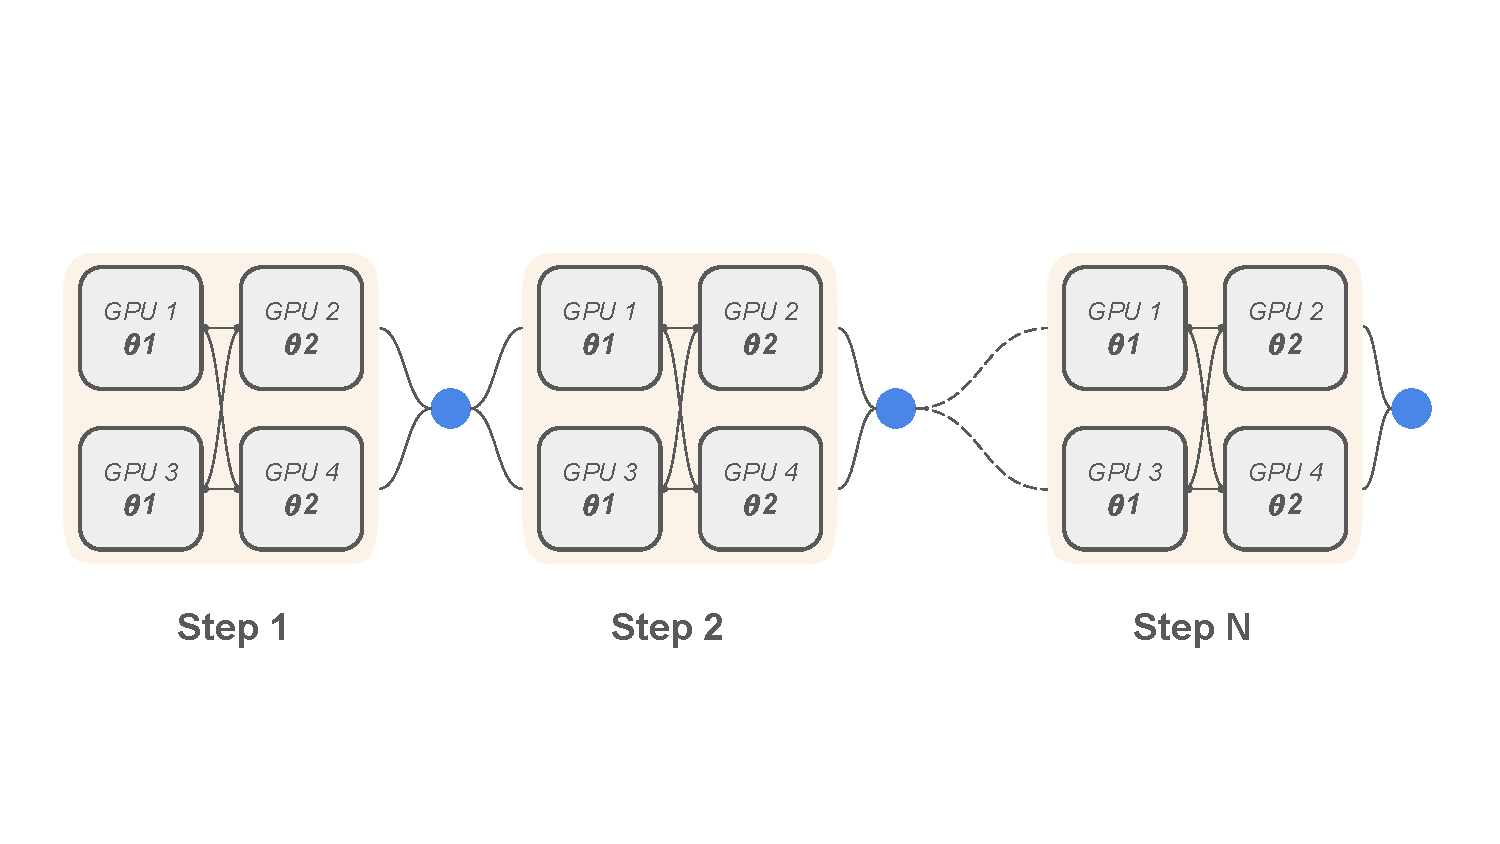
\includegraphics[width=0.45\textwidth]{figures/swarm.pdf}
    \caption{\textbf{SWARM.} We visualize the communication patterns of SWARM
    for $9$ nodes in $3\times 3$ SWARM. In SWARM, nodes forward activations and
    gradients in a stochastic manner, forming DP groups after the forward and
    backward passes are complete.}
    \label{fig:swarm}
\end{figure}

\section{DiLoCo-SWARM}

SWARM enables large-scale, fault-tolerant DPP training in decentral settings.
However, one of its two major communication pattern relies on costly
synchronization of gradients at every step. Meanwhile, DiLoCo has proven a
robust alternative to step-synchronous gradient synchronization in a variety of
settings, but, on its own, hits natural memory limitations at larger scale.

This motivates DiLoCo-SWARM: a decentralized training method combining the best
of both worlds. It reduces the communication cost incurred by gradient
synchronization via DiLoCo while preserving the desirable scaling and
fault-tolerance properties of SWARM. Put simply, it replaces DP groups with
DiLoCo groups, as visualized in Figure~\ref{fig:diloco-swarm}.

\begin{figure}[ht]
    \centering
    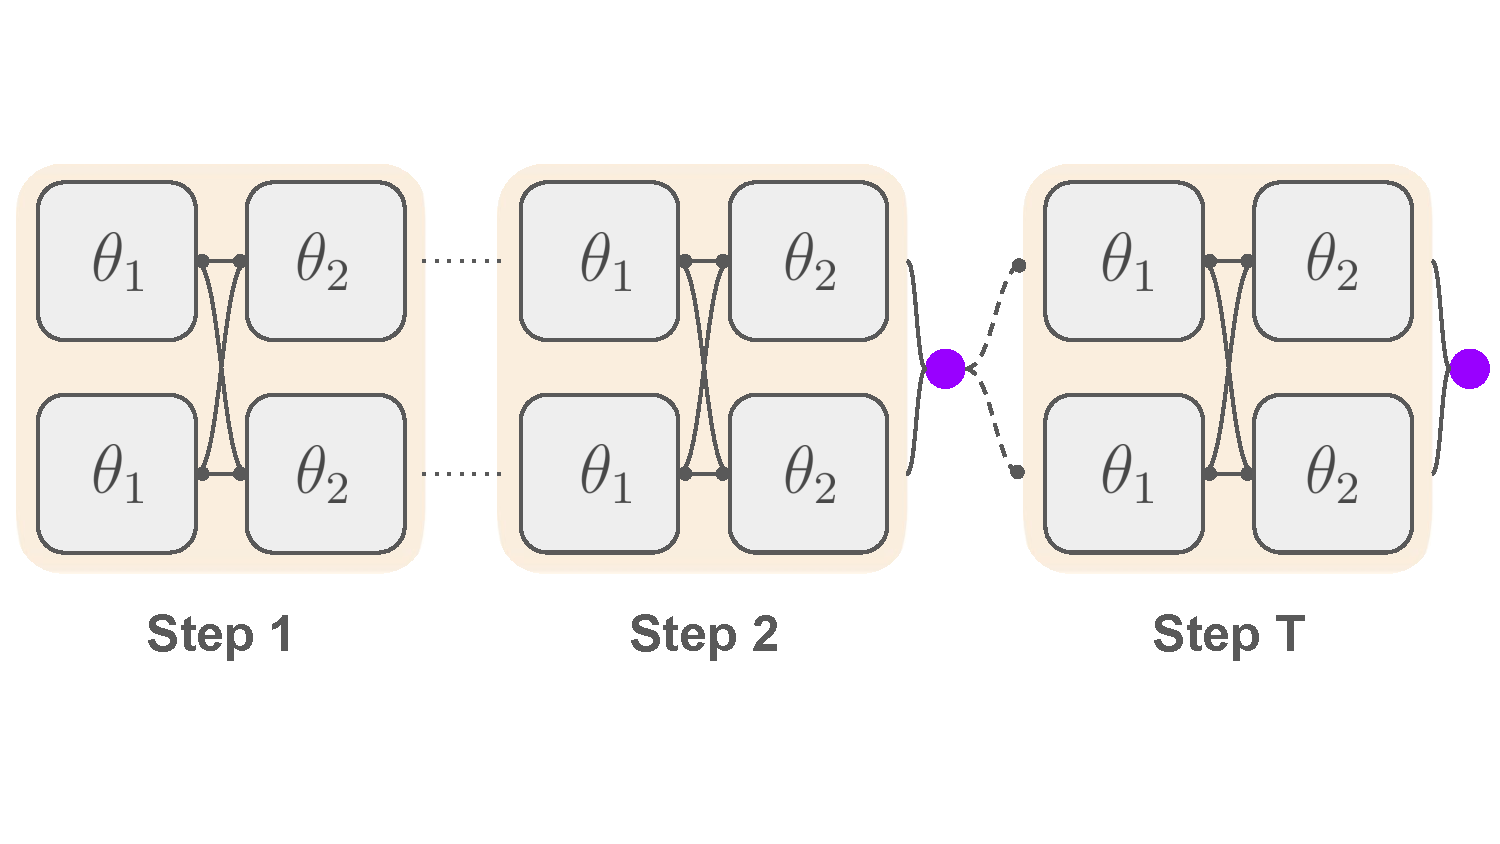
\includegraphics[width=0.45\textwidth]{figures/diloco-swarm.pdf}
    \caption{\textbf{DiLoCo-SWARM.} We visualize the communication patterns of
    DiLoCo-SWARM for $9$ nodes in $3\times 3$ DiLoCo-SWARM. In comparison to
    regular SWARM, DiLoCo-SWARM replaces DP groups with DiLoCo groups which
    synchronize less frequently.}
    \label{fig:diloco-swarm}
\end{figure}

\subsection{Algorithm}

Algorithm~\ref{alg:diloco-swarm} describes the algorithmic details of
DiLoCo-SWARM. We assume a $m\times n$ grid of nodes for simplified notation
without loss of generality, but note that SWARM, and therefore DiLoCo-SWARM, can
handle any number of nodes per stage. DiLoCo-SWARM proceeds as follows: At the
start of an inner optimization loop, each node in a SWARM stage shares the same
global model shard $\theta_j^{(t-1)}$. Then, SWARM nodes perform $H$ local
steps. At each local step, nodes compute a local gradient $g_{i,j}$ by
stochastically forwarding activations and gradients to peers in adjacent stages,
and update their local model shard $\theta_{i,j}^{(t-1)}$ via a local optimizer
$\mathtt{OPT}_{L}$. After the inner optimization loop completes, nodes within a
SWARM stage form DiLoCo groups. They compute a local pseudo-gradient
$\Delta_{i,j} = \theta_{i,j}^{(t-1)} - \theta_j^{(t-1)}$ and synchronize them to
update their global model shard $\theta_j^{(t)}$ using the global optimizer
$\mathtt{OPT}_{G}$.

Note, that the algorithm description largely follows SWARM for accumulating
gradients during local steps, and DiLoCo for gradient synchronization.  Also,
observe that because of stochastic wiring gradients $g_{i,j}$ may depend on
batches $x_i'$ sampled from different data shards, leading to "mixing" of data
shards across nodes.

\begin{algorithm}
\caption{DiLoCo-SWARM}
\label{alg:diloco-swarm}
\begin{algorithmic}[1]
\State \textbf{Input:} Data shard $D_i$, Model shard $\theta_j$, Loss $\mathcal{L}$, Optimizers $\mathtt{OPT}_{L}$ and $\mathtt{OPT}_{G}$, Num. Local Steps $H$
\Procedure{FwdBwd}{}
  \If{$j = 1$} \Comment{First stage}
    \State Sample batch: $x_i \sim D_i$
      \State Forward: $a_{i,1} \gets f^{(1)}_{\theta_{i,1}}(x_i)$
      \State Send forward: $\mathtt{send}(a_{i,1}, 2)$ 
      \State Receive backward: $g_{i,2} \gets \mathtt{recv}(1)$
      \State Compute gradient: $g_{i,1} \gets g_{i,2} \cdot \nabla_{\theta_j} f^{(j)}_{\theta_j}(a_{i,j-1})$
  \ElsIf{$j = n$} \Comment{Last stage}
      \State Receive forward: $a_{i,n-1} \gets \mathtt{recv}(n-1)$
      \State Compute gradient: $g_{i,n} \gets \nabla_{\theta_n} \mathcal{L}(a_{i,n-1})$
      \State Send backward: $\mathtt{send}(g_{i,n}, n-1)$
  \Else \Comment{Intermediate stages}
      \State Receive forward: $a_{i,j-1} \gets \mathtt{recv}(j-1)$
      \State Forward: $a_{i,j} \gets f^{(j)}_{\theta_j}(a_{i,j-1})$
      \State Send forward: $\mathtt{send}(a_{i,j}, j+1)$
      \State Receive backward: $g_{i,j+1} \gets \mathtt{recv}(j+1)$
      \State Compute gradient: $g_{i,j} \gets g_{i,j+1} \cdot \nabla_{\theta_j} f^{(j)}_{\theta_j}(a_{i,j-1})$
      \State Send backward: $\mathtt{send}(g_{i,j}, j-1)$
  \EndIf
  \Return $g_{i,j}$
\EndProcedure
\State Copy global model: $\theta_{ij}^{(t-1)} \gets \theta_j^{(t-1)}$
\For{$H$ steps}
  \State Compute gradients: $g_{i,j} \gets \mathtt{FwdBwd}()$
  \State Update local model: $\theta_{ij}^{(t-1)} \gets \mathtt{OPT}_{L}(\theta_{ij}^{(t-1)}, g_{i,j})$
\EndFor
\State Compute pseudo-gradient: $\Delta_{i,j} \gets \theta_{ij}^{(t-1)} - \theta_j^{(t-1)}$
\State Sync pseudo-gradients: $\Delta_j \gets \frac{1}{m}\sum_j^m \Delta_{i,j}$
\State Update global model: $\theta_j^{(t)} \gets \mathtt{OPT}_{G}(\theta_j^{(t-1)}, \Delta_j)$
\end{algorithmic}
\end{algorithm}

\subsection{Implementation}

A key contribution of this work is the release of the full experiment codebase
(\github{}) and a distilled single-file training script (\gist{}) which
implements all mentioned distributed training methods in one place, i.e. DP, PP,
DPP, SWARM, with optional DiLoCo-style gradient synchronization. Example
invocations are shown in the Appendix.

% Advantages (Minimal, PyTorch-only, various algos, HF support)
The implementation is designed with simplicity and readability in mind. It only
depends on PyTorch, specifically the \texttt{torch.distributed} package, for
training and communication. Further, instead of multiple thousand lines of code 
of the original SWARM implementation, it uses only a few hundred. Put together,
this makes it easy for anybody to understand various traditional parallelization
techniques, and how they interact with decentralized variants, like DiLoCo and
SWARM. To enable quick testing and debugging, it can emulate nodes via threads.
Finally, it integrates with HuggingFace for models and datasets, allowing
diverse testing setups. In summary, we hope that the training script will be an
excellent educational resource, and the full experiment codebase a good starting
point for quickly verifying and iterating on research ideas, as evidenced by
DiLoCo-SWARM.

% Limitations (Not feature-complete and less efficient)
The simplicity comes at the cost of efficiency and feature-incompleteness. In
particular, a subset of SWARM features, most notably those enabling
fault-tolerance, are not yet supported. Some require features beyond what is
supported in PyTorch today. A full list of not-yet supported features is listed
in the Appendix. An important consequence of this is that the script currently
only supports runs on a single node with multiple local workers, and is
therefore best-suited for research purposes. Finally, the training script does
not optimize pipeline scheduling, and overlaying computation and communication,
and so time-to-accuracy comparison between methods are not meaningful.

% NanoGPT
The implementation should therefore be seen as a supplemental resource other
open-source implementations of SWARM and DiLoCo, focusing on simplicity and
hackability. Our hope is that it might trigger similar effects as other
open-source efforts like NanoGPT~\cite{karpathy2024nanogpt}, a minimal
re-implementation of GPT-2, which today is the default within the open-source
community to benchmark architecture, hyper-parameter and optimizer research in
an open and reproducible manner~\cite{moddednanogpt2024}.

\section{Experiments}

% Introduction
In this section we report the experiment setup and results validating
DiLoCo-SWARM. The setup and hyperparameters largely follow the
DiLoCo~\cite{douillard2023diloco} experiments.

% Dataset
We consider a language modeling task on the FineWeb-Edu~\cite{penedo2024fineweb}
dataset, a large pre-training dataset consisting of high-quality web pages
filtered for educational content. We choose this dataset over other common
pre-training datasets due to its high token efficiency allowing to match the
original GPT-2 performance on the HellaSwag~\cite{zellers2019hellaswag}
benchmark when training the same model with 10x less
data~\cite{karpathy2024nanogpt}.

% Model
For all experiments, we use the GPT-2 family of models~\cite{radford2019gpt2} in
varying sizes. We adapt the original architectural hyperparameters to match the
original GPT-2 paper~\cite{radford2019gpt2}, as shown in Table~\ref{tab:models}.
Notice that the parameter counts slightly deviate from the original paper, since
we do not share the weights of the embedding matrix and language modeling head
to circumvent additional gradient communication in pipelined settings between
the first and last stage. Per default, we train GPT-2 Small and train from
scratch.

% Model sizes
\begin{table}[h]
\centering
\begin{tabular}{lcccc}
\toprule
\textbf{Model} & \textbf{Layers} & \textbf{Heads} & \textbf{Hidden Size} & \textbf{Params} \\
\midrule
Tiny & 4 & 4 & 128 & $\sim$14M \\
Small & 12 & 12 & 768 & $\sim$180M \\
Medium & 24 & 16 & 1024 & $\sim$405M \\
Large & 36 & 20 & 1280 & $\sim$800M \\
\bottomrule
\end{tabular}
\caption{\textbf{Model Sizes.} GPT-2 model configurations used in experiments.
Parameter counts account for non-shared weights of embedding matrix and language
modeling head.}
\label{tab:models}
\end{table}

% Hyper-parameters
The hyper-parameters are adapted from the tuning done in
DiLoCo~\cite{douillard2023diloco}: The default local optimizer is
AdamW~\cite{loshchilov2019adamw} with a linearly warmed up learning rate of
$4\cdot 10^{-4}$, and a weight decay of $0.01$. When DiLoCo is active, we use a
Nesterov with a learning rate of $0.7$ and a momentum of $0.9$ as the global
optimizer. A detailed description of the hyperparameters is provided in
Table~\ref{tab:hyperparameters} in the Appendix.

% Evaluation
Our main evaluation metric is the perplexity on a held-out validation set of 10M
randomly sampled tokens from FineWeb-Edu. We evaluate during and after training
to show the convergence against the number of training steps, as well as the
total communication cost.

% Main Experiment: DiLoCo-SWARM
\textbf{Main Experiment.} Our main experiment setup closely follows that of
DiLoCo~\cite{douillard2023diloco}. We train two baselines and a DiLoCo-SWARM.
The weak baseline trains for 2,000 steps on one GPU with a batch size of 512 and
sequence length of 1024, for a total data budget of 1B tokens. The strong
baseline is a 4x2 SWARM, i.e. eight workers distributed evenly into two pipeline
stages. This baseline performs regular gradient synchronization at every step.
The higher compute budget is used to scale the batch size to the number of nodes
per stage, leading to a total training budget of 4B tokens. Finally, we train a
4x2 DiLoCo-SWARM which is identical to the strong baseline but performs outer
optimization steps every 50 steps.

\begin{figure*}[t]
  \centering
  \begin{subfigure}[b]{0.48\textwidth}
    \centering
    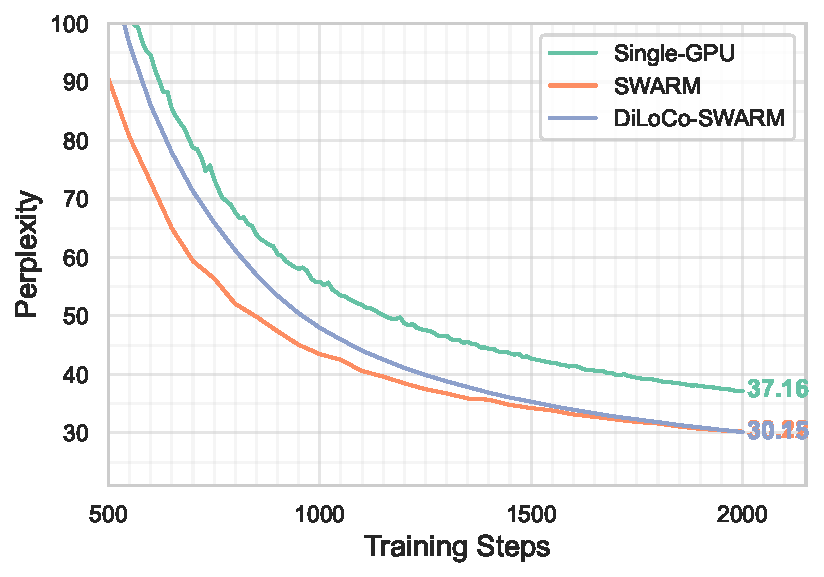
\includegraphics[width=\textwidth]{figures/experiment1-1.pdf}
    \caption{Training Steps}
    \label{fig:experiment1-1}
  \end{subfigure}
  \hfill
  \begin{subfigure}[b]{0.48\textwidth}
    \centering
    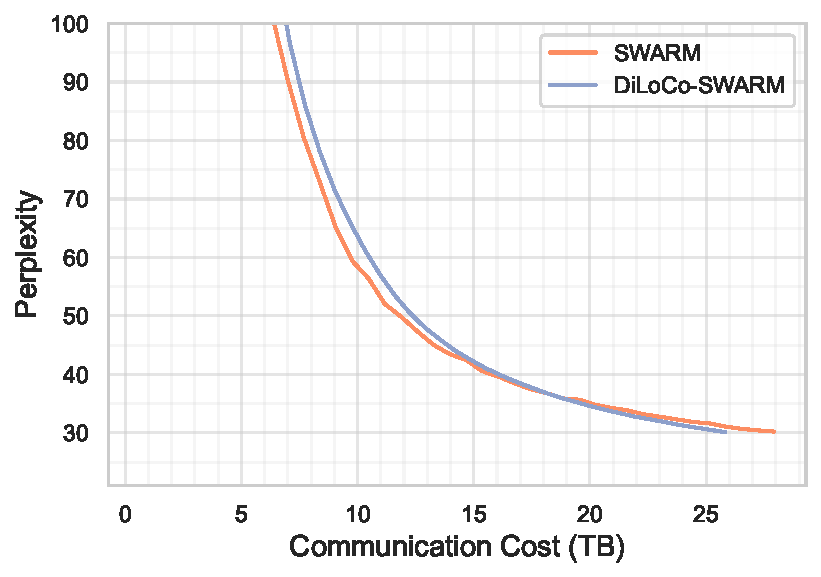
\includegraphics[width=\textwidth]{figures/experiment1-2.pdf}
    \caption{Communication Cost}
    \label{fig:experiment1-2}
  \end{subfigure}
  \caption{\textbf{Main Result} We show the validation perplexity against the
  number of training steps (left) and the total communication cost (right) for
  two baselines and SWARM-DiLoCo. With the same compute and data budget but with
  50x less gradient synchronization, DiLoCo-SWARM matches the generalization
  performance of the strong SWARM baseline. However, the total communication
  cost is only insignificantly reduced, as the cost is dominated by PP
  communication for GPT-2 Small.}
  \label{fig:experiment1}
\end{figure*}

Figure~\ref{fig:experiment1-1} shows the validation perplexity as a function of
the training steps. Unsurprisingly, the weaker baseline, using less compute and
data, is outperformed by the stronger SWARM baseline with final perplexities of 
37.16 and 30.22, respectively. Our main finding is that DiLoCo-SWARM closely
matches, and even exceeds, the strong baseline in generalization performance
with a validation perplexity of 30.15, despite synchronizing gradients 50x fewer
times. This implies that DiLoCo-style gradient synchronization is compatible
with SWARM parallelism, allowing to reduce the communication cost incurred by 
gradient synchronization within pipeline stages of SWARM.

Figure~\ref{fig:experiment1-2} shows the total communication cost for the same
experiments. Surprisingly, the total communication cost is only moderately
reduced in DiLoCo-SWARM compared to SWARM. This finding points at a an important
difference between DiLoCo and DiLoCo-SWARM. In DiLoCo, synchronizing gradients
every $H$ translates to a directly proportional reduction in communication cost
by $1/H$. DiLoCo-SWARM, in contrast, interleaves DP and PP communication. Since
DiLoCo can only reduce DP communication cost, the PP communication stays
constant.  Hence, we can only hope to reduce the total communication cost as a
factor of $1/H \cdot \text{DP Communication Cost Fraction}$. Luckily, the
square-cube law~\cite{ryabinin2023swarm} suggests that the PP communication cost
scales quadratically while DP communication scales cubically with increasing
model sizes. Thus, with larger models, DP communication dominates the total
communication cost. We illustrate this phenomenon in
Figure~\ref{fig:square-cube-law}, which shows the fraction of the communication
cost incurred by DP and PP communication for 4x2 SWARMs training increasingily
large models. In summary, DP communication dominates the total communication
cost for larger models, and so DiLoCo-SWARM is only able to reduce the
communication cost by a factor of $1/H$ in the limit of large models.

\begin{figure}[ht]
  \centering
  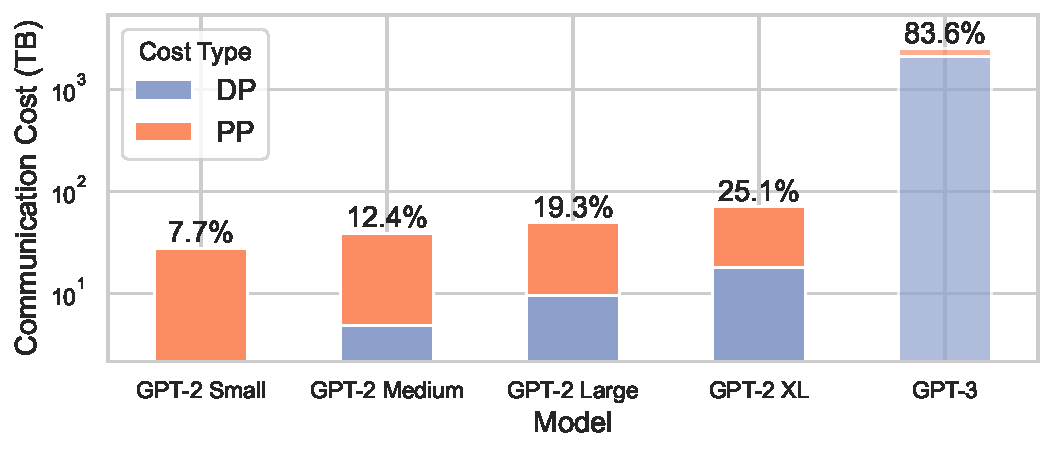
\includegraphics[width=0.45\textwidth]{figures/square-cube-law.pdf}
  \caption{\textbf{Communication Cost Scaling} We show the communication cost
  incurred by DP and PP communication for 4x2 SWARMs in our common training
  setup.  For small models, PP communication dominates the total communication
  cost. However, for larger models, DP communication dominates the total
  communication cost.} 
  \label{fig:square-cube-law}
\end{figure}


% Experiment 2: Ablation on communication frequency
\textbf{Communication Frequency.} We are interested in how \textit{infrequently}
gradient synchronization can occur within SWARM pipeline stages without
impacting convergence. Intuitively, the slower the frequency, the worse
convergence, but whether synchronizing every 10 or 200 steps negatively impacts
performance, has implications on the practical usefulness of the algorithm. To
investigate, we train five models using the same training setup and only vary
the number of local training steps before performing synchronizing gradients.

% TODO: Add perplexities in legend
% \begin{figure}[ht]
%   \centering
%   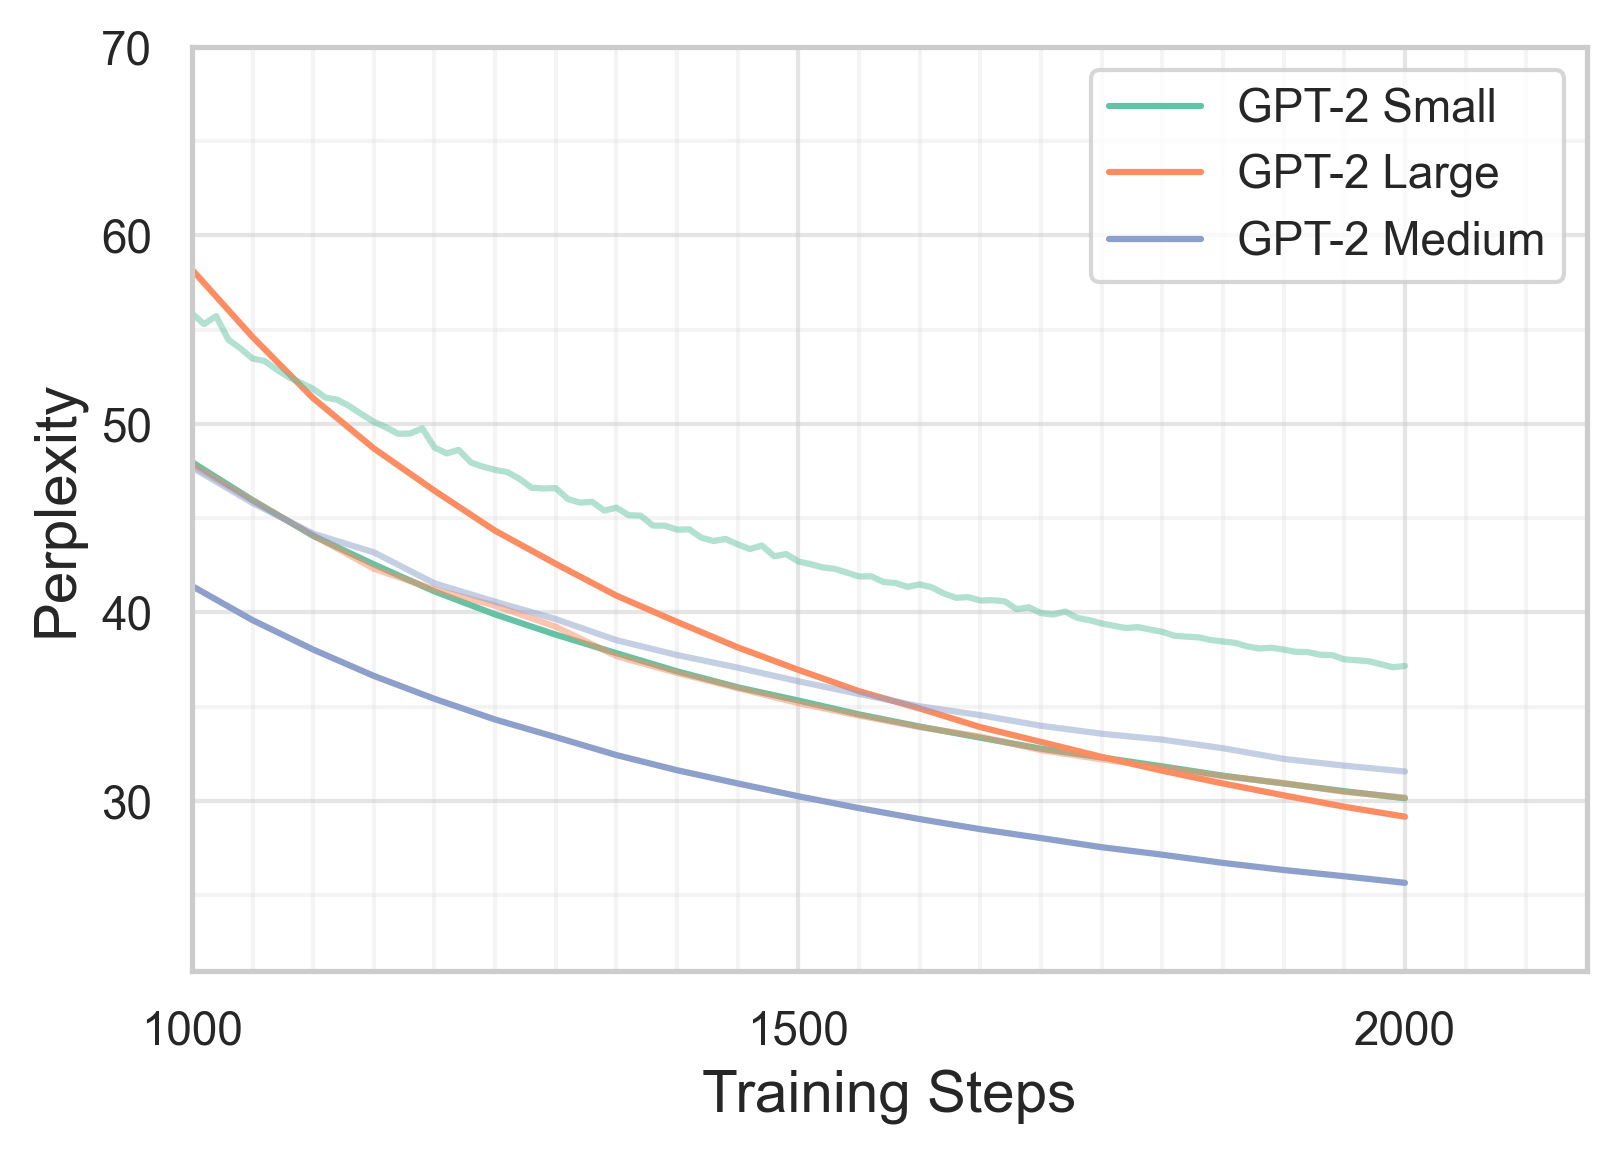
\includegraphics[width=0.45\textwidth]{figures/experiment3.png}
%   \caption{\textbf{Communication Frequency} We vary the number of local training
%   steps before performing an outer optimization step from $\{10, 20, 50, 100, 200\}$ 
%   and report the validation perplexity throughout training. Synchronizing more
%   frequently yields better results but performance degradation is neglibible even
%   on all tested values.}
%   \label{fig:experiment2}
% \end{figure}

Table~\ref{tab:experiment2} shows the results of this experiment. In line with
the original DiLoCo results, generalization performance monotonically increases
with higher gradient synchronization frequency. However, the performance
degradation for less frequent gradient synchronization is mild. Synchronizing
every 10 steps achieves the best performance, with a validation perplexity of
27.95. Note, that this also significantly out-performs the SWARM baseline in
Figure~\ref{fig:experiment1} while still reducing the synchronization frequency
by 10x. In our experiments, a good trade-off between communication frequency and
performance is achieved when synchronizing every 50 steps, which is therefore
used throughout all other experiments.

\begin{table}[ht]
\centering
\begin{tabular}{lccc}
\toprule
\textbf{Freq.} & \textbf{Val. PPL} & \textbf{$\Delta$ (Abs./Rel.)} \\ 
\midrule
10 & 27.95 & - \\
20 & 28.61 & 0.66 / 2.36\% \\
50 & 30.15 & 2.2 / 7.87\% \\
100 & 30.49 & 2.54 / 9.09\% \\
200 & 31.27 & 3.32 / 11.88\% \\
\bottomrule
\end{tabular}
\caption{\textbf{Communication Frequency} We report the final validation
perplexity for different communication frequencies and their absolute and
relative changes compared to synchronizing every 10 steps.}
\label{tab:experiment2}
\end{table}

% Experiment 3: Varying the model size
\textbf{Model Sizes.} Finally, we train three sizes of GPT-2 models, as 
described in Table~\ref{tab:models} to assess whether DiLoCo-style gradient
synchronization is robust scaling the model. We use the same hyper-parameters
for all models from Table~\ref{tab:hyperparameters} and train for 2,000 steps.
For each size, we also train a single-node baseline with four times smaller
batch size.

\begin{figure}[ht]
  \centering
  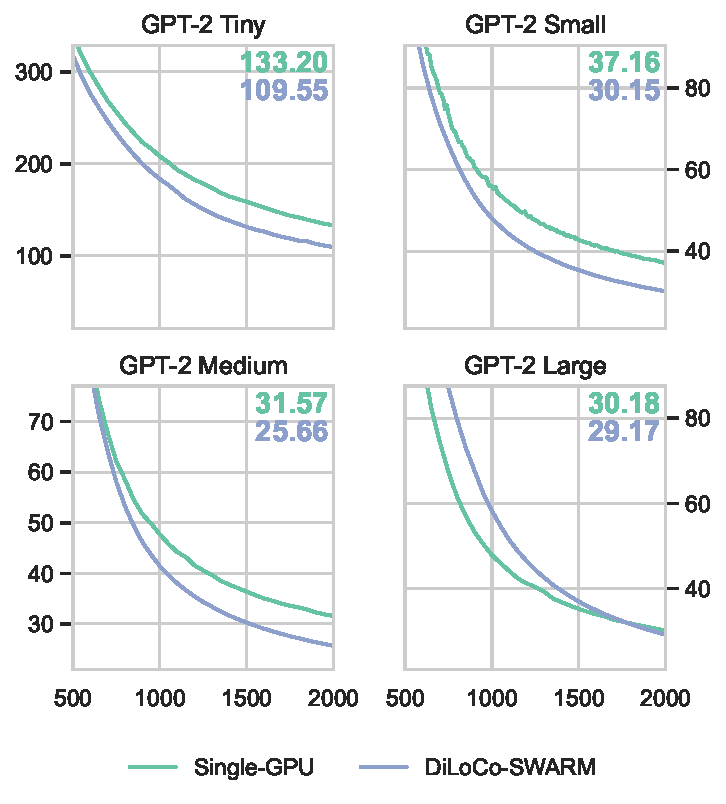
\includegraphics[width=0.48\textwidth]{figures/experiment3.pdf}
  \caption{\textbf{Model Size} We train three different sizes of GPT-2 models and report the validation perplexity throughout training. The performance improvement over the single-node baseline remains constant at around 18\% across all model sizes, suggesting that DiLoCo-style gradient synchronization scales well with increasing model size.}
  \label{fig:experiment3}
\end{figure}

% \begin{table}[ht]
% \centering
% \begin{tabular}{lccc}
% \toprule
% \textbf{\# Params} & \textbf{PPL} & \textbf{$\Delta$ (Abs./Rel.)} \\ 
% \midrule
% 180M & 30.15 & 7.01 / 18.86\% \\
% 400M & 25.66 & 5.91 / 18.72\% \\
% 800M & & & \\
% \bottomrule
% \end{tabular}
% \caption{\textbf{Model Size} We report the final validation perplexity for
% different model sizes and their absolute and relative changes compared to a
% single-node baseline with smaller batch size.}
% \label{tab:experiment3}
% \end{table}

Table~\ref{tab:experiment3} shows with DiLoCo we obtain a constant improvement
of $\sim$18\% over the single-node baseline run, for all tested model sizes.
This finding suggests that gradient synchronization with DiLoCo scales to larger
models sizes. This is an important finding as SWARM is designed to train models
which do not naively fit into a single nodes' memory and the scaling properties
of DiLoCo are hence crucial.

\section{Conclusion}

The results of this study suggest that DiLoCo-style gradient synchronization is
compatible with SWARM parallelism. This implies that gradient 
synchronization via a dual optimization scheme is an effective tool for gradient
synchronization, even when the gradients correspond to model shards in pipeline
stages accumulated via stochastic forward and backward passes.

These findings have implications both for the SWARM and DiLoCo community. For
SWARM, this means that the communication cost incurred by gradient
synchronization within pipeline stages can be drastically reduced. Hence, future
research and open-source efforts should focus on integrating DiLoCo-style 
gradient synchronization into production implementations of SWARM. For DiLoCo,
the findings further underline the robustness of the method, suggesting that
DiLoCo is a good candidate as a drop-in replacement anytime gradients need to be
synchronized between nodes in distributed settings.

\section{Limitations}

Several limitations to this work should be noted.

% Environment
All experiments were conducted on co-located GPUs with reliable and fast
interconnectivity. The initial premise of this research, however, was the
decentralized setting with unreliable, heterogeneous and poorly connected
compute resources. SWARM is only favourable over traditional parallelization
techniques in this setting, and so while the experiments in this study suggest
that DiLoCo-style gradient synchronization can be used in SWARM, it remains to
show how the method behaves in a truly decentral setting when scaled to larger
models, requiring more pipeline stages and nodes per stage.

% No tuning
Another limitation of this work is the lack of hyper-parameter tuning. All
hyper-parameters are copied from the tuned parameters in
DiLoCo~\cite{douillard2023diloco}. This might not always be fair, and lead to
pessimistic estimates of the validaiton performance. However, due to the
similarity of models, datasets, and training algorithms, we believe they are a
good proxy. Regardless, a sensible continuation of this work would be to
validate the results with tuned hyper-parameters.

% Scale
Moreover, it should be noted that the original DiLoCo and SWARM experiments were
conducted on larger scale. Both train on a data budget of roughly 50B tokens per
run, resulting in multiple GPU days worth of compute. Such resources were simply
not available within the scope of this project but is required to obtain robust
results on the efficacy of the algorithm.

% Efficiency
All of the above point to more more scale and compute. A crucial step is to
integrate optimized implementations of DiLoCo and SWARM, including efficient
pipeline scheduling techniques, allowing for fault-tolerant training over-the-
internt. Only then, experiments can be conducted on truly larger scale and in a
realistic environment. A particularly interesting question is how the reduced
communication frequency of gradients impacts the wall-clock runtime of the
algorithm in different network settings and for various model sizes.

% Different SWARM structures
Finally, another interesting, but open, research question is how the
DiLoCo-SWARM behaves when varying the number of workers per stage. The current
implementation does not scale beyond co-located GPUs, so investigating this
question requires implementing peer-to-peer communication over the Internet.

\section*{Acknowledgements}
\label{sec:acknowledgements}

This work was developed in collaboration with the Scalable Computing Systems
(SaCS) lab at EPFL as well as Prime Intellect. All compute was kindly sponsored
by Prime Intellect.

% Bibliography
\bibliography{references}
\bibliographystyle{icml2023}

% Appendix
\newpage
\appendix
\onecolumn

\section{Appendix}

% TODO: Supported and non-supported features in implementation

\subsection{Training Script Invocations}

Below we show example invocations for different distributed training algorithms.
All examples use a GPT-2 small model and the FineWeb-Edu dataset as an example.
For more details see the README on \github.

\begin{lstlisting}[language=bash]
# Single GPU training
torchrun --nproc_per_node 1 src/train.py --swarm.num_stages 1 \
    --model @configs/model/gpt2-small.toml \
    --data @configs/data/fineweb-edu-10bt.toml
\end{lstlisting}

\begin{lstlisting}[language=bash]
# Pipeline parallel training with 2 GPUs
torchrun --nproc_per_node 2 src/train.py --swarm.num_stages 2 \
    --model @configs/model/gpt2-small.toml \
    --data @configs/data/fineweb-edu-10bt.toml
\end{lstlisting}

\begin{lstlisting}[language=bash]
# Data parallel training with 2 GPUs
torchrun --nproc_per_node 2 src/train.py --swarm.num_stages 2 \
    --model @configs/model/gpt2-small.toml \
    --data @configs/data/fineweb-edu-10bt.toml
\end{lstlisting}

\begin{lstlisting}[language=bash]
# DiLoCo training with 2 GPUs
torchrun --nproc_per_node 2 src/train.py --swarm.num_stages 2 \
    --train.outer_optimizer @configs/optimizer/nesterov.toml
    --model @configs/model/gpt2-small.toml \
    --data @configs/data/fineweb-edu-10bt.toml
\end{lstlisting}

\begin{lstlisting}[language=bash]
# SWARM training with 4 GPUs
torchrun --nproc_per_node 4 src/train.py --swarm.num_stages 2 \
    --model @configs/model/gpt2-small.toml \
    --data @configs/data/fineweb-edu-10bt.toml
\end{lstlisting}

\begin{lstlisting}[language=bash]
# DiLoCo-SWARM training with 4 GPUs
torchrun --nproc_per_node 4 src/train.py --swarm.num_stages 2 \
    --train.outer_optimizer configs/optimizer/nesterov.toml
    --model @configs/model/gpt2-small.toml \
    --data @configs/data/fineweb-edu-10bt.toml
\end{lstlisting}

% Hyperparameters
\subsection{Hyperparameters}

Table~\ref{tab:hyperparameters} shows the hyperparameters used throughout the
experiments. The outer optimizer parameters is only used for DiLoCo-style
training, else the gradients are averaged before performing a regular optimizer
step by default.

\begin{table}[ht]
\centering
\begin{tabular}{llc}
\toprule
\textbf{Hyperparameter} & \textbf{Value} \\ 
\midrule
\multirow{1}{*}{General} & Batch Size & 512 \\ 
& Sequence Length & 1024 \\ 
& Steps & 2000 \\
\hline
\multirow{1}{*}{InnerOptimizer} & Name & AdamW \\ 
& Weight decay & - \\ 
& Learning Rate & $4 \times 10^{-4}$ \\ 
\hline
\multirow{1}{*}{OuterOptimizer} & Name & Nesterov \\ 
& Learning Rate & 0.7 \\ 
& Momentum & 0.9 \\ 
\bottomrule
\end{tabular}
\caption{Hyperparameters}
\label{tab:hyperparameters}
\end{table}

% Hardware
\subsection{Hardware}

All experiments were conducted on a single node with eight co-located H100 GPUs
on \href{https://app.primeintellect.com/}{Prime Intellect Compute}.

\end{document}